\section{Introduction}

Energy-efficiency is an important goal to lower carbon-dioxide emissions of deep neural network (DNN) driven applications and is a critical prerequisite to enable applications in edge computing.
\emph{DNN accelerators}, \ie, specialized hardware for inference, are used to reduce and limit energy consumption alongside cost and space compared to mainstream hardware, \eg, GPUs.
These accelerators generally feature on-chip SRAM used as scratchpads, \eg, to store DNN weights. Data access/movement
constitutes a dominant component of accelerator energy consumption \cite{SzeIEEE2017}.
Reduced precision \cite{LinICML2016} is a widely used measure to reduce energy consumption at the cost of \emph{approximate computing} \cite{SampsonPLDI2011}.
Recently, DNN accelerators \cite{ReagenISCA2016, KimDATE2018,ChandramoorthyHPCA2019} further lower memory supply voltage to increase energy efficiency since dynamic power varies quadratically with voltage. However, aggressive SRAM supply voltage scaling, causes bit-level failures in SRAM on account of process variation \cite{GanapathyDAC2017,GuoJSSC2009} with direct impact on the stored DNN weights. The rate $p$ of these errors increases exponentially with lowered voltage
and causes devastating drops in DNN accuracy such that memory reliability becomes the bottleneck in realizing low power DNN accelerators. In this paper, we aim to enable very low-voltage operation of DNN accelerators by developing DNNs robust to such bit errors in their weights, allowing DNN inference on \emph{``approximate hardware''} \cite{KoppulaMICRO2019,SampsonPLDI2011}. This is also desirable to improve security against adversarial
manipulation of voltage settings \cite{TangUSENIX2017}. 
In general, robustness to bit errors in DNNs is a desirable goal in order to maintain safe operation and should become a standard performance metric in low power DNN design.

\figref{fig:introduction} shows the average bit error rates of SRAM arrays as supply voltage is aggressively scaled below \Vmin, \ie, the measured lowest voltage at which there are no bit errors. Voltage (x-axis) and energy ({\color{colorbrewer1}red}, right y-axis) are normalized \wrt \Vmin and the energy per access at \Vmin, respectively. DNNs robust to a bit error rate ({\color{colorbrewer2}blue}, left y-axis) of, \eg, $p = 1\%$ allow to reduce SRAM energy by roughly $30\%$.
To improve DNN robustness to bit errors, we first consider the impact of fixed-point quantization on robustness. While prior work \cite{MurthyARXIV2019,MerollaARXIV2016,SungARXIV2015} studies robustness \emph{to} quantization, the impact of random bit errors \emph{in} quantized weights has not been considered so far. We find that the choice of quantization scheme has tremendous impact on robustness, even though accuracy is not affected. In particular, we identify a particularly \textbf{robust quantization scheme}, \Quant in \figref{fig:contributions} ({\color{colorbrewer1}red}). 
Additionally, independent of the quantization scheme, we propose aggressive \textbf{weight clipping} during training. This acts as an explicit regularizer leading to spread out weight distributions, improving
robustness significantly,
\Clipping in \figref{fig:contributions} ({\color{colorbrewer2}blue}). This is in contrast to, \eg, \cite{ZhuangCVPR2018,SungARXIV2015} ignoring weight outliers to reduce quantization range, with sole focus of improving accuracy.

\begin{figure}[t]
    \centering
    \vspace*{-0.1cm}
    \hspace*{-0.4cm}
    \begin{subfigure}{0.475\textwidth}
    	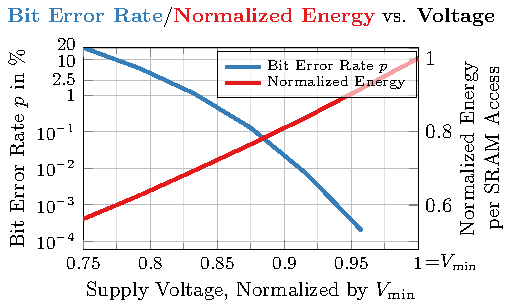
\includegraphics[height=5.25cm]{c10_intro2.pdf}
    \end{subfigure}
    \vspace*{-8px}
    \caption{
    \textbf{Energy and Low-Voltage Operation.} Average bit error rate $p$ ({\color{colorbrewer2}blue}, left y-axis) from $32$ 14nm SRAM arrays of size $512{\times}64$ from \cite{ChandramoorthyHPCA2019} and energy ({\color{colorbrewer1}red}, right y-axis) vs. voltage (x-axis). Voltage is normalized by \Vmin, the minimal measured voltage for error-free operation, as well as the energy per SRAM access at \Vmin. SRAM accesses have significant impact on the DNN accelerator's energy \cite{ChenISCA2016}. Reducing voltage leads to exponentially increasing bit error rates.
    }
    \label{fig:introduction}
    \vspace*{-0.2cm}
\end{figure}

Common error correcting codes (ECCs such as SECDED), cannot correct \emph{multiple} bit errors per word (containing multiple DNN weights). However, for $p = 1\%$, the probability of two or more bit errors in a $64$-bit word is $13.5\%$.
Error detection via redundancy \cite{ReagenISCA2016} or supply voltage boosting \cite{ChandramoorthyHPCA2019} allow error-free low-voltage operation at the cost of additional energy or space. Therefore, \cite{KimDATE2018} proposes a co-design approach of training DNNs on \emph{profiled} SRAM bit errors. Similarly, for approximate DRAMs, \cite{KoppulaMICRO2019} combines profiled bit error training with a clever weight to DRAM mapping. These approaches work as the spatial bit error patterns can be assumed fixed for a \emph{fixed} accelerator \emph{and} voltage. The bit error pattern is obtained by post-silicon profiling and characterization of memories.
The random nature of variation-induced bit errors requires profiling to be carried out for each voltage, memory array and individual chip in order to obtain the corresponding bit error patterns. This makes training DNNs on profiled bit error patterns an expensive process. More importantly, we demonstrate that the obtained DNNs do \emph{not} generalize across voltages or to unseen bit error patterns, \eg, from other memory arrays. 
We propose \textbf{random bit error training (\Random)} which, in combination with weight clipping and robust quantization, obtains robustness against completely \emph{random} bit error patterns, see  \figref{fig:contributions} ({\color{colorbrewer4}violet}). Thereby, it generalizes across chips \emph{and} voltages, without any profiling, hardware-specific data mapping or other circuit-level mitigation strategies.

\begin{figure}[t]
	\centering
	\vspace*{-0.1cm}
	\hspace*{-0.25cm}
	\begin{subfigure}{0.425\textwidth}
         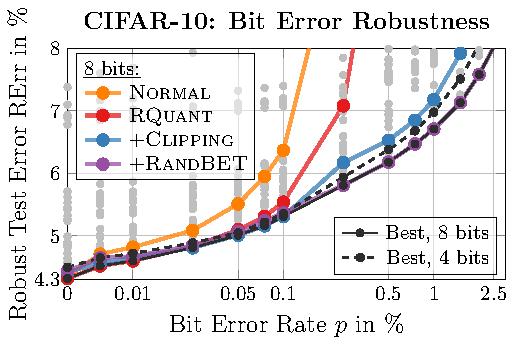
\includegraphics[height=5.25cm]{c10_contributions_8bit}
    \end{subfigure}
    \vspace*{-8px}
    \caption{
    \textbf{Robustness to Random Bit Errors.} Robust test error (test error \emph{after} injecting bit errors, \RTE, lower is better $\downarrow$, y-axis) plotted against bit error rate $p$ (x-axis). Robustness to higher bit error rates allows more energy efficient operation, \cf \figref{fig:introduction}. For $8$ bit, through robust quantization (\Quant, {\color{colorbrewer1}red}), additionally weight clipping (\Clipping, {\color{colorbrewer2}blue}) and finally adding random bit error training (\Random, {\color{colorbrewer4}violet}) robustness improves significantly. 
    The Pareto optimal frontier is shown for $8$ bit (black solid) and $4$ bit (dashed) quantization.
    }
    \label{fig:contributions}
    \vspace*{-0.2cm}
\end{figure} 

\textbf{Contributions:}
We combine our \textbf{robust fixed-point quantization \Quant}, \ie, reduced quantization range and robust implementation, with \textbf{weight clipping} and \textbf{random bit error training (\Random)} in order to obtain high robustness against low-voltage induced, random bit errors. We consider fixed-point quantization schemes in terms of robustness \emph{and} accuracy, instead of \emph{solely} focusing on accuracy as related work. Furthermore, we show that aggressive weight clipping, as regularization during training, is an effective strategy to improve robustness through redundancy. In contrast to \cite{KimDATE2018,KoppulaMICRO2019}, the robustness obtained through \Random generalizes across chips \emph{and} voltages, as evaluated on profiled SRAM bit error patterns from \cite{ChandramoorthyHPCA2019}. 
Finally, we discuss the involved trade-offs regarding robustness and accuracy and make our code publicly available to facilitate research in this highly applicable area of DNN robustness. \figref{fig:contributions} highlights key results on \CifarT: with $8$ bit and an increase in test error of less than $1\%$, roughly $20\%$ energy savings are possible. Combined with low-precision, \eg, for $4$ bit quantization, $30\%$ energy savings are possible at $p = 1\%$ with an increase in error rate of less than $2.5\%$. 

\begin{figure*}
	\centering
	\vspace*{-0.1cm}
	\begin{tikzpicture}
		\node[anchor=north west] at (0,0){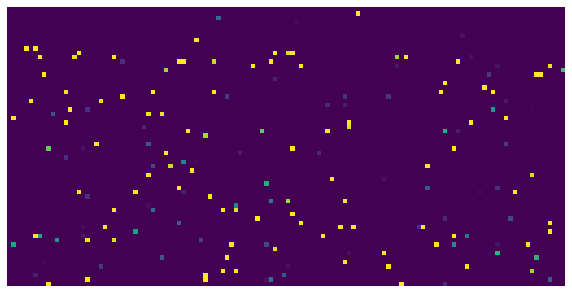
\includegraphics[width=4cm]{errors_18_3}};
		\node[anchor=north west] at (4,0){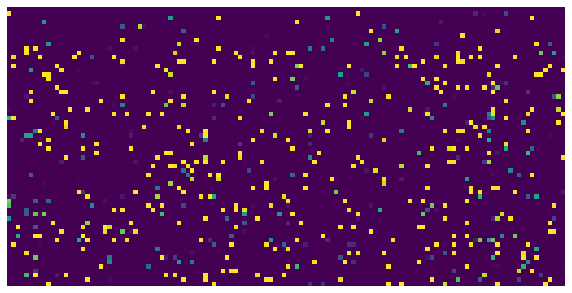
\includegraphics[width=4cm]{errors_18_2}};
		\node[anchor=north west] at (8,0){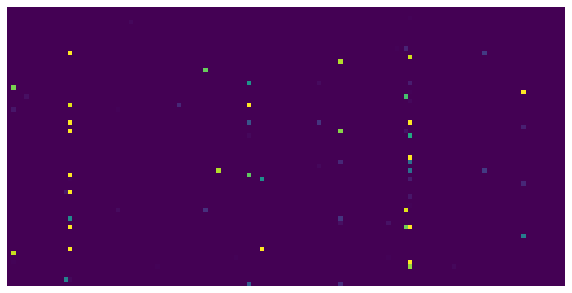
\includegraphics[width=4cm]{errors_n_3}};
		\node[anchor=north west] at (12,0){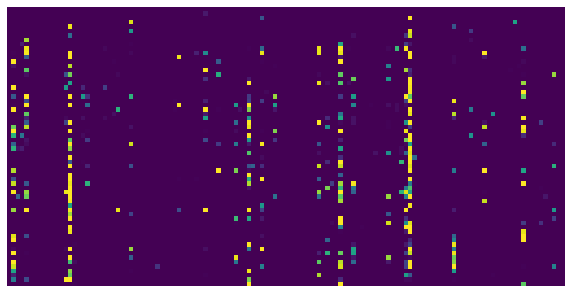
\includegraphics[width=4cm]{errors_n_2}};
		
		\node[anchor=south east,fill opacity=0.75,fill=white] at (4, -2){$p{\approx}0.86\%$};
		\node[anchor=south east,fill opacity=0.75,fill=white] at (8, -2){$p{\approx}2.75\%$};
		\node[anchor=south east,fill opacity=0.75,fill=white] at (12, -2){$p{\approx}0.14\%$};
		\node[anchor=south east,fill opacity=0.75,fill=white] at (16, -2){$p{\approx}1.08\%$};
		
		\draw[white!30!black,-, line width=0.75pt] (8.125,-2.4) -- (8.125,0.4);
		\draw[thick,->] (0.05,0.05) -- (1,0.05);
		\draw[thick,->] (-0.05,-0.05) -- (-0.05,-1);
		\node[anchor=south] at (0.75,0.05){128 columns};
		\node[rotate=90,anchor=south] at (-0.05,-0.6){64 rows};
		
		\node[anchor=south] at (4,-0.15) {\bfseries Chip 1};
		\node[anchor=south] at (12,-0.15) {\bfseries Chip 2};
		
		\draw[thick,->] (2.5,-2.8) -- (4.5,-2.8) node[anchor=west] {bit error rate $p$ increases};
		\draw[thick,->] (2.5,-2.4) -- (4.5,-2.4) node[anchor=west] {voltage decreases};
		
		\draw[thick,-] (9.75, -2.2) -- (9.75,-2.4) -- (10.75,-2.4);
		\node[anchor=west] at (10.75, -2.4){bit errors subset of};
		\draw[thick,->] (13.75,-2.4) -- (14.75,-2.4) -- (14.75, -2.2);
	\end{tikzpicture}
	\vspace*{-8px}
	\caption{\textbf{Exemplary SRAM Bit Error Patterns.} Measured bit errors from two chips with on-chip SRAM (left and right), showing bit flip probability for a segment of size $64 \times 128$ bits: {\color{yellow!75!black}yellow} indicates a bit flip probability of one, {\color{violet}violet} indicates zero probability. We show measurements corresponding to two supply voltages. %(right lower than left)
	With lower voltage, bit error rate increases. Also, the bit errors for higher voltage (= lower bit error rate) are a subset of those for lower voltage (= higher rate), \cf \secref{sec:errors}. Our error model randomly distributes bit errors across space. However, as example, we also show SRAM chip 2 which has a different spatial distribution with bit errors distributed along columns. We aim to obtain robustness across different memory arrays, voltages \emph{and} allowing arbitrary DNN weight to memory mappings.}
	\label{fig:errors}
\end{figure*}

\textbf{Outline:} We review related work in \secref{sec:related-work} and provide a detailed description and discussion of the considered low-voltage bit error model in \secref{sec:errors}. In \secref{sec:robustness}, we discuss fixed-point quantization and its influence on bit error robustness and present weight clipping and \Random as effective strategies to improve robustness. Finally, \secref{sec:experiments} includes our experimental results. We conclude in \secref{sec:conclusion}.